\chapter{Spannungsverteilung in luftgek"uhlten Transformatoren\label{chapter:thema}}
\lhead{Spannungsverteilung in luftgekühlten Transformatoren}
\begin{refsection}
\chapterauthor{Reto Christen}

\section{Einleitung}

Heutzutage werden elektronische Betriebsmittel mittels CAD-Programme berechnet und ausgelegt. Dies ermöglicht eine einfache und kostengünstige Entwicklung sowie Herstellung, da der erste Prototyp die Erwartungen meistens bereits erfüllt. Die Lösungen von CAD-Programmen, was nichts anderes als Lösungen von partiellen oder gewöhnlichen Differentialgleichungen sind, ergeben neue Herausforderungen, wie beispielsweise in der Numerik. 

In diesem Kapitel wird ein solches Problem vorgestellt, genauer betrachtet und schlussendlich gelöst.

\section{Problemstellung}

Luftgekühlte Transformatoren sind im Gegensatz zu ölgekühlten Transformatoren eher gefährdet Teilentladungen oder gar Durchschläge zu haben. Dies liegt daran, dass die Isolationsfestigkeit von Luft wesentlich schlechter als in Öl ist. Da ein luftgekühlter Transformator im Gegensatz zu einem ölgekühlten Transformator diverse Vorteile besitzt, ist es von Interesse, die elektrischen Felder so zu limitieren, damit Durchschläge und grösstenteils auch Teilentladungen verhindert werden können. 

Früher wurde ein Transformator oder allgemein ein elektronisches Betriebsmittel nach Erfahrungen gebaut. Dabei war es Gang und Gäbe, dass es mehrere Prototypen brauchte, bis die ersten Spannungsprüfungen bestanden werden konnten. Deshalb sind CAD-Simulationen wesentlich schneller und vor allem kostengünstiger. Das Ziel soll es sein, der Transformator möglichst genau darzustellen und dessen Spannungsverteilung zu berechnen, denn die Spannung und die Geometrie zusammen ergeben das elektrische Feld, welches schlussendlich zu Durchschlägen oder Teilentladungen führt.

An der Hochschule für Technik Rapperswil wurde am Institut für Energietechnik eine Methode entwickelt, wie ein Blitzstoss Spannungsimpuls möglichst genau simuliert werden kann \cite{trafo:BILImpulse}. Dies Methode funktioniert sehr gut für Leistungstransformatoren und konnte mit Messungen auch verifiziert werden. 
Will dieses Prinzip aber auf Instrumententransformatoren angewendet werden, ergibt die wesentlich höhere Anzahl von Wicklungen und deren engeren Lagen nummerische Probleme im Lösungsverfahren. 

Diese Probleme werden nun Schrittweise behandelt und bestmöglich gelöst. 


\subsection{Ersatzschaltbild}
Ein Transformator, ob öl- oder luftgekühlt, kann prinzipiell mit dem Ersatzschaltbild \ref{trafo:einfaches_ESB} dargestellt werden. Dies macht Sinn, wenn der Transformator als Ganzes dargestellt werden will. Da bei diesem Problem aber die inneren Spannungen relevant sind, kann dieses bereits bekannte Ersatzschaltbild nicht verwendet werden. Es gilt nun, ein neues und genaueres Ersatzschaltbild zu finden. 

\begin{figure}
	\centering
	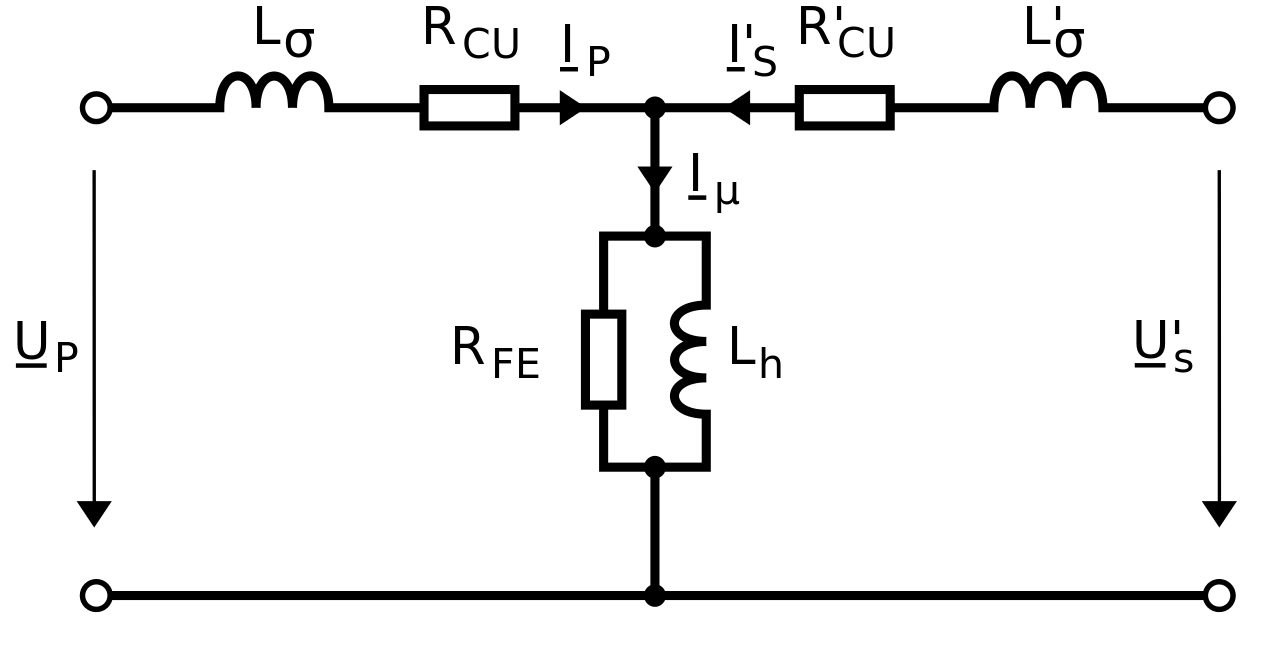
\includegraphics[width=0.5\textwidth]{trafo/Einfaches_ESB.png}
	\caption[Einfach Ersatzschaltbild für einen Transformator]{Einfach Ersatzschaltbild für einen Transformator.}
	\label{trafo:einfaches_ESB}
\end{figure}

Ein Ansatz ist es, jede Wicklung einzeln zu modellieren. Pro Windung wird ein elektrischer Widerstand sowie Induktivität in Serie geschaltet. Ebenfalls müssen die Kapazitäten sowie die Leitfähigkeiten gegenüber Masse und den übrigen Windungen berücksichtigt werden \cite{trafo:BILImpulse}. 

Dieses Ersatzschaltbild wird in der Abbildung \ref{trafo:erweitertes_ESB} dargestellt. Als Beispiel wird ein kleines Transformator Beispiel, bestehend aus 4 Windungen, verwendet. Mit Messungen an Testtransformatoren zeigte sich, das ab ca. 20 Windungen die Simulationen mit diesem Ersatzschaltbild sehr genau übereinstimmen. 

\begin{figure}
	\centering
	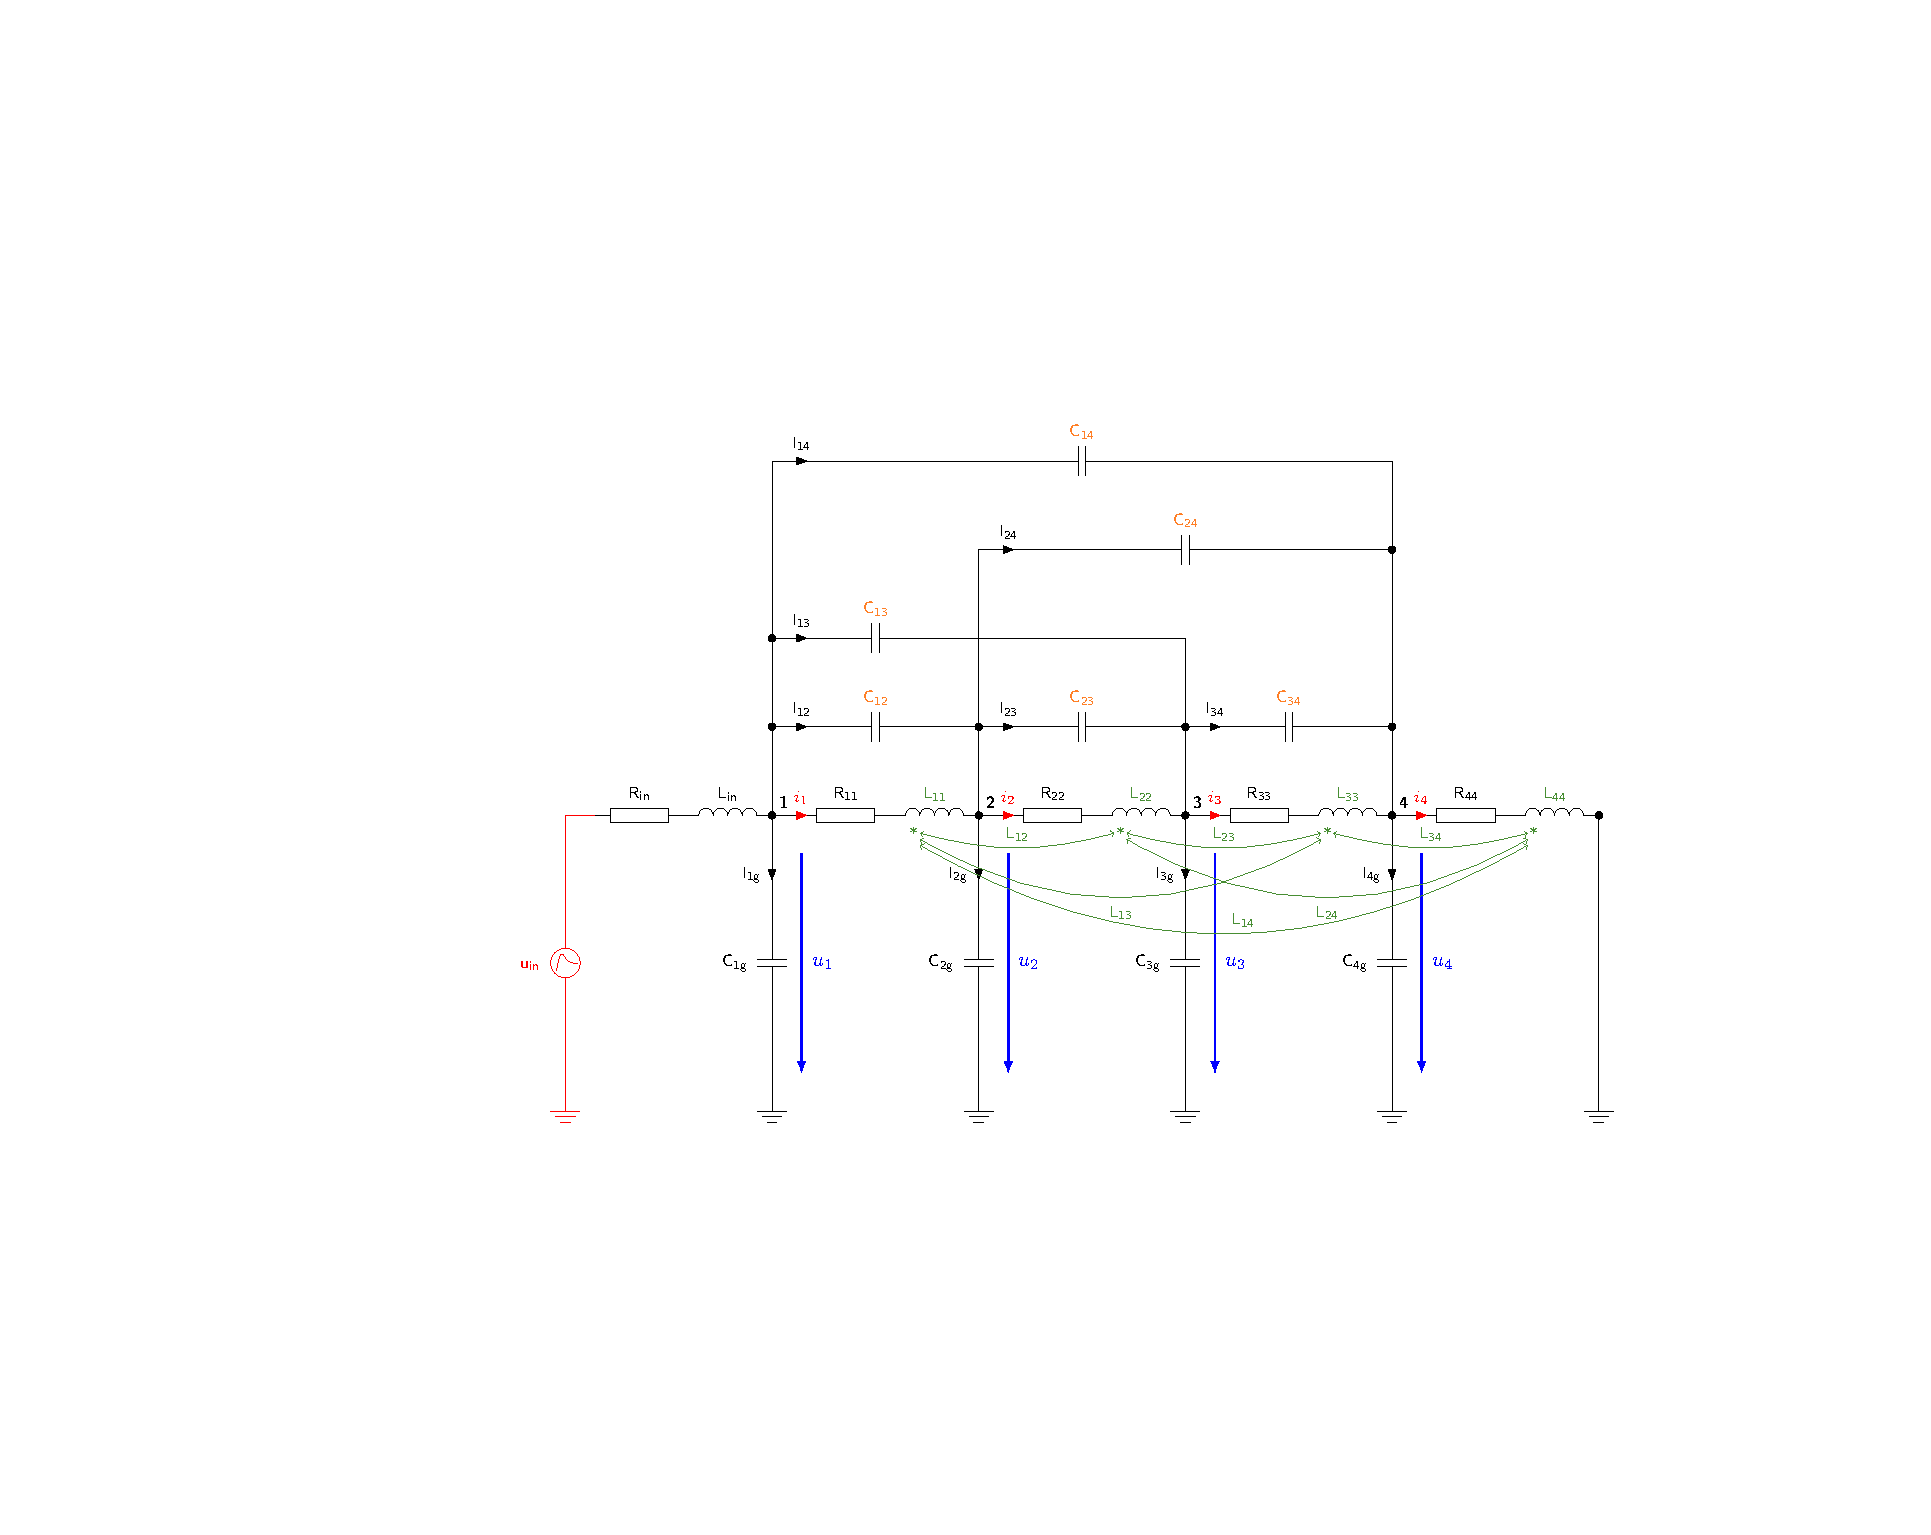
\includegraphics[width=0.8\textwidth]{trafo/Trafo_Modell.pdf}
	\caption[Erweitertes Ersatzschaltbild für einen Transformator]{Erweitertes Ersatzschaltbild für einen Transformator mit 4 Wicklungen. Die Leitwerte zwischen den Wicklungen und gegenüber Masse sind auf Grund der Übersichtlichkeit weggelassen worden. Die grünen Pfeile stellen die Mitkopplung der Spulen dar. }
	\label{trafo:erweitertes_ESB}
\end{figure}

Damit die Werte der einzelnen Elementen ermittelt werden können, sind Finite-Element-Methode-(FEM)-Simulationen in einem CAD Programm notwendig. Alle Wicklungen abgesehen einer werden auf das Spannungspotential \SI{0}{\volt} gesetzt. Die aktuelle gemessene Wicklung wird hingegen auf das Potential von \SI{1}{\volt} gesetzt und anschliessend werden die Induktivitäten sowie Kapazitäten gegenüber allen anderen Wicklungen ermittelt.


\section{Mathematische Lösung}
\subsection{Differentialgleichung}

Es gilt nun eine Differentialgleichung für das gefundene Ersatzschaltbild aufzustellen. Mittels dem Maschensatz (blaue Pfeile) und der Knotenpunktregel (rote Punkte) können die Differentialgleichungen pro Wicklung aufgestellt werden (dargestellt in \ref{trafo:orig}).

\begin{figure}
	\centering
	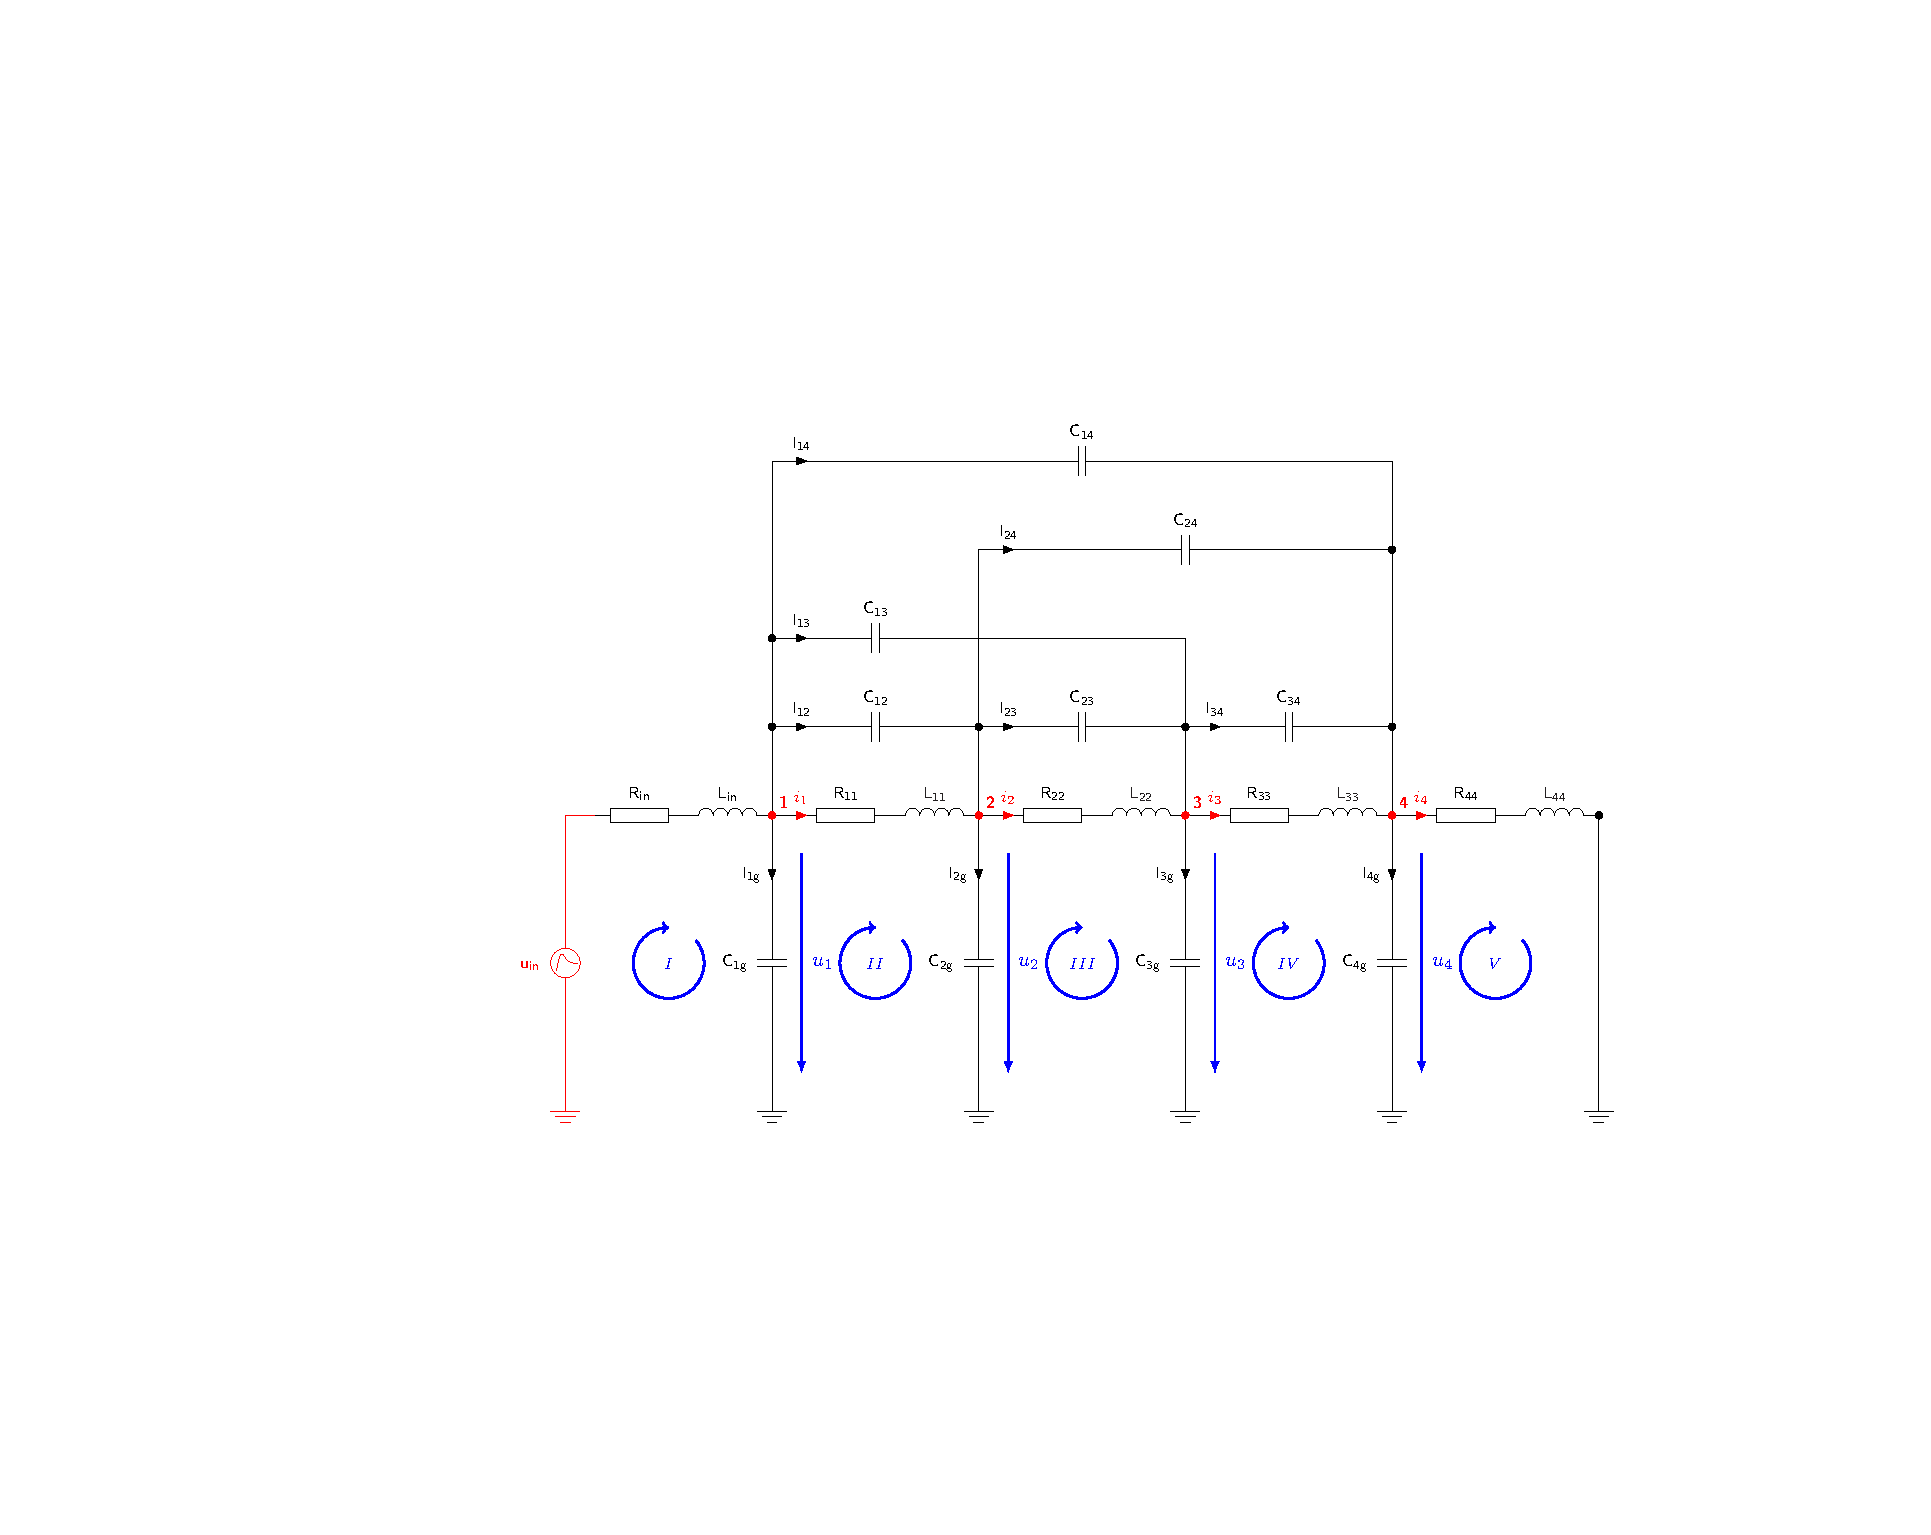
\includegraphics[width=0.8\textwidth]{trafo/orig_trafo.pdf}
	\caption[Erweitertes Ersatzschaltbild für einen Transformator mit Maschensatz und Knotenpunkt]{Erweitertes Ersatzschaltbild für einen Transformator mit 4 Wicklungen. Die blaue Pfeilen stellen den Maschensatz und die roten Punkte den Knotenpunktregel dar.}
	\label{trafo:orig}
\end{figure}

Beispielsweise kann die Gleichungen der Wicklung 1 als 

\begin{equation*}
	u_\mathrm{Rin} + u_\mathrm{Lin} + u_1 = u_\mathrm{in}
\end{equation*}
und 
\begin{equation}
	i_\mathrm{in} = i_1 + i_{C1g} + i_{R12} + i_{C12} + i_{R13} + i_{C13} + i_{R14} + i_{C14}
\end{equation}
geschrieben werden. 

Mit etwas Umformungen kann der ganze Transformator als System mehreren Differentialgleichungen geschrieben werden \cite{trafo:SeminarCHR}. Als Beispiel wird wiederum der Transformator mit 4 Windungen gewählt. Der Vektor $E$ ist der Störterm, sprich in diesem Falle der Blitzstoss, des Systemes.

{\footnotesize 
\begin{align}
			&
			\underbrace{\begin{bmatrix}
			L_\mathrm{in}&0&0&0&0 & 0&0&0&0 \\
			0&L_{11}&L_{12}&L_{13}&L_{14} & 0&0&0&0 \\
			0&L_{21}&L_{22}&L_{23}&L_{24} & 0&0&0&0 \\
			0&L_{31}&L_{32}&L_{33}&L_{34} & 0&0&0&0 \\
			0&L_{41}&L_{42}&L_{43}&L_{44} & 0&0&0&0 \\
			0&0&0&0&0 & \sum{C_{1x}}&-C_{12}&-C_{13}&-C_{14} \\
			0&0&0&0&0 & -C_{21}&\sum{C_{2x}}&-C_{23}&-C_{24} \\
			0&0&0&0&0 & -C_{31}&-C_{32}&\sum{C_{3x}}&-C_{34} \\
			0&0&0&0&0 & -C_{41}&-C_{42}&-C_{43}&\sum{C_{4x}}
			    \end{bmatrix}}_{\text{$M$}}
			\cdot
			\underbrace{\begin{bmatrix}
			\frac{di_\mathrm{in}}{dt} \\
			\frac{di_1}{dt} \\
			\frac{di_2}{dt} \\
			\frac{di_3}{dt} \\
			\frac{di_4}{dt} \\
			\frac{du_1}{dt} \\
			\frac{du_2}{dt} \\
			\frac{du_3}{dt} \\
			\frac{du_4}{dt}
			\end{bmatrix}}_{\text{$\dot{x}$}}
			= \nonumber \\
			&
			\underbrace{\begin{bmatrix}
			-R_\mathrm{in}&0&0&0&0 & -1&0&0&0 \\
			0&-R_{11}&0&0&0 & 1&-1&0&0 \\
			0&0&-R_{22}&0&0 & 0&1&-1&0 \\
			0&0&0&-R_{33}&0 & 0&0&1&-1 \\
			0&0&0&0&-R_{44} & 0&0&0&1 \\
			1&-1&0&0&0 & -\sum G_{1x}&G_{12}&G_{13}&G_{14} \\
			0&1&-1&0&0 & G_{21} &- \sum G_{2x}& G_{23}& G_{24} \\
			0&0&1&-1&0 & G_{31} & G_{32} &-\sum G_{3x}&G_{34} \\
			0&0&0&1&-1 & G_{41}&G_{42}&G_{43}&-\sum G_{4x}
			\end{bmatrix}}_{\text{$F$}}
			\cdot
			\underbrace{\begin{bmatrix}
			i_\mathrm{in} \\
			i_1 \\
			i_2 \\
			i_3 \\
			i_4 \\
			u_1 \\
			u_2 \\
			u_3 \\
			u_4
			\end{bmatrix}}_{\text{$x$}}
			+
			\underbrace{\begin{bmatrix}
			u_\mathrm{in} \\
			0 \\
			0 \\
			0 \\
			0 \\
			0 \\
			0 \\
			0 \\
			0
			\end{bmatrix}}_{\text{$E$}}
			\label{trafo:DGL}
\end{align}
}
		


Die Matrix $M$ ist eine symmetrische Matrix, welches für weitere Berechnungen wesentliche Vorteile mit sich bringt. Die Matrix $N$ ist fast symmetrisch. Wenn der Maschensatz jedoch in die andere Richtung wie in Abbildung \ref{trafo:orig} angewendet wird, lässt sich auch diese Matrix mit fast keinem Aufwand symmetrisch machen. Dies ist für dieses Beispiel zwar nicht nötig, trotzdem kann es für andere Lösungsansätze von Vorteil sein. Aus der Gleichung \ref{trafo:DGL} wird nun 

{\footnotesize 
\begin{align}
			&
			\underbrace{\begin{bmatrix}
			\color{red}-\color{black}L_\mathrm{in}&0&0&0&0 & 0&0&0&0 \\
			0&\color{red}-\color{black}L_{11}&\color{red}-\color{black}L_{12}&\color{red}-\color{black}L_{13}&\color{red}-\color{black}L_{14} & 0&0&0&0 \\
			0&\color{red}-\color{black}L_{21}&\color{red}-\color{black}L_{22}&\color{red}-\color{black}L_{23}&\color{red}-\color{black}L_{24} & 0&0&0&0 \\
			0&\color{red}-\color{black}L_{31}&\color{red}-\color{black}L_{32}&\color{red}-\color{black}L_{33}&\color{red}-\color{black}L_{34} & 0&0&0&0 \\
			0&\color{red}-\color{black}L_{41}&\color{red}-\color{black}L_{42}&\color{red}-\color{black}L_{43}&\color{red}-\color{black}L_{44} & 0&0&0&0 \\
			0&0&0&0&0 & \sum{C_{1x}}&-C_{12}&-C_{13}&-C_{14} \\
			0&0&0&0&0 & -C_{21}&\sum{C_{2x}}&-C_{23}&-C_{24} \\
			0&0&0&0&0 & -C_{31}&-C_{32}&\sum{C_{3x}}&-C_{34} \\
			0&0&0&0&0 & -C_{41}&-C_{42}&-C_{43}&\sum{C_{4x}}
			    \end{bmatrix}}_{\text{$M$}}
			\cdot
			\underbrace{\begin{bmatrix}
			\frac{di_\mathrm{in}}{dt} \\
			\frac{di_1}{dt} \\
			\frac{di_2}{dt} \\
			\frac{di_3}{dt} \\
			\frac{di_4}{dt} \\
			\frac{du_1}{dt} \\
			\frac{du_2}{dt} \\
			\frac{du_3}{dt} \\
			\frac{du_4}{dt}
			\end{bmatrix}}_{\text{$\dot{x}$}}
			= \nonumber \\
			&
			\underbrace{\begin{bmatrix}
			\color{red}+\color{black}R_\mathrm{in}&0&0&0&0 & \color{red}+\color{black}1&0&0&0 \\
			0&\color{red}+\color{black}R_{11}&0&0&0 & \color{red}-\color{black}1&\color{red}+\color{black}1&0&0 \\
			0&0&\color{red}+\color{black}R_{22}&0&0 & 0&\color{red}-\color{black}1&\color{red}+\color{black}1&0 \\
			0&0&0&\color{red}+\color{black}R_{33}&0 & 0&0&\color{red}-\color{black}1&\color{red}+\color{black}1 \\
			0&0&0&0&\color{red}+\color{black}R_{44} & 0&0&0&\color{red}-\color{black}1 \\
			1&-1&0&0&0 & -\sum G_{1x}&G_{12}&G_{13}&G_{14} \\
			0&1&-1&0&0 & G_{21} &- \sum G_{2x}& G_{23}& G_{24} \\
			0&0&1&-1&0 & G_{31} & G_{32} &-\sum G_{3x}&G_{34} \\
			0&0&0&1&-1 & G_{41}&G_{42}&G_{43}&-\sum G_{4x}
			\end{bmatrix}}_{\text{$N$}}
			\cdot
			\underbrace{\begin{bmatrix}
			i_\mathrm{in} \\
			i_1 \\
			i_2 \\
			i_3 \\
			i_4 \\
			u_1 \\
			u_2 \\
			u_3 \\
			u_4
			\end{bmatrix}}_{\text{$x$}}
			+
			\underbrace{\begin{bmatrix}
			u_\mathrm{in} \\
			0 \\
			0 \\
			0 \\
			0 \\
			0 \\
			0 \\
			0 \\
			0
			\end{bmatrix}}_{\text{$E$}}
			\label{trafo:symmetricalDGL}
\end{align}
}

Dieses System mehrere Differentialgleichungen kann auch mit Matrizen und Vektoren geschrieben werden, welches sich etwas übersichtlicher darstellen lässt. 

\begin{equation}
	M \cdot \dot x = N \cdot x + E
	\label{trafo:matricesDGL}
\end{equation}

Wird die Massenmatrix $M$ auf die rechte Seite der Gleichung \ref{trafo:matricesDGL} dividiert, ergibt dies

\begin{equation}
	\dot{x} = M^{-1} \cdot N \cdot x + M^{-1} \cdot E = A \cdot x + B
\end{equation}
welches die allgemein bekannte und auch lösbare Zustandsraumdarstellung \index{Zustandsraumdarstellung} ist (engl. state space).

Das Problem scheint bereits gelöst zu sein, insofern sich die Massenmatrix \textbf{M} invertieren lässt. In der Theorie wäre dies tatsächlich auch machbar, jedoch sehr aufwändig. Weil auch gewisse Eigenwerte zu klein sind, explodiert die Lösung und kann somit mit diesem Ansatz nicht gelöst werden.

Folglich muss ein Ansatz gefunden werden, welcher die Massenmatrix $M$ möglichst rechenzeitschonend invertiert und die Eigenwerte der Inversion im Griff hat. 


\subsection{Singular Value Decomposition (SVD) \index{Singular Value Decomposition}}

\subsection{Exaktes Lösungsverfahren}

\subsection{Schrittweite und Fehlerterm}

\subsection{Optimierungen}

\section{Anwendung der gefundenen Lösungen}

\printbibliography[heading=subbibliography]
\end{refsection}
